\section{Neuronale Netze}
Ein Neuron ist ein Schwingkreis. Es hat n Eingänge und einen Ausgang. Die Werte der
Eingänge werden summiert. Wenn die Summe der Eingänge einen Schwellwert übertrifft, wechselt der Ausgang, das Neuron feuert.
Für die Schwellwertfunktion, wird entweder die Signum (0/1) oder die Sigmoid-Funktion welche ``weiche'' Kanten hat und ableitbar ist verwendet.
\begin{figure}[htb]
	\centering
	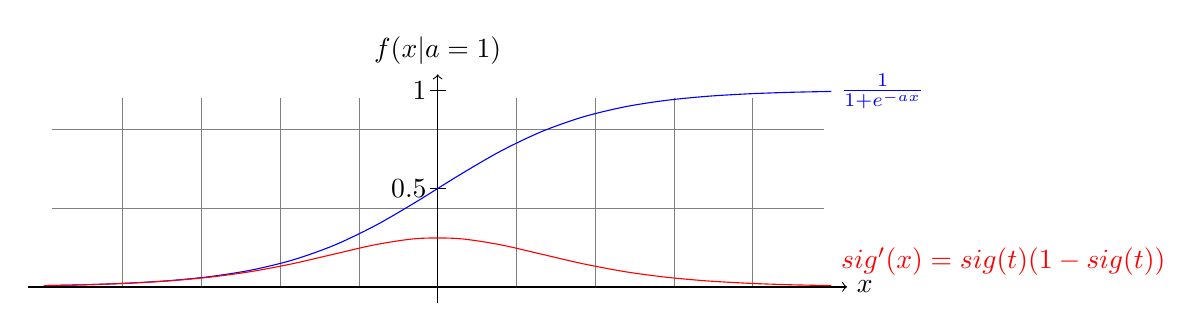
\begin{tikzpicture}[domain=-5:5, smooth, samples=20]
	\draw[very thin, color=gray] (-4.9,0.0) grid (4.9,2.4);

	\draw[->] (-5.2,0) -- (5.2,0) node[right] {$x$};
	\draw[->] (0,-0.2) -- (0,2.7) node[above] {$f(x|a=1)$};
	\draw (-0.1,2.5) --(0.1,2.5) node [left] {$1~$};
	\draw (-0.1,1.25) -- (0.1,1.25) node [left] {$0.5~$};

	\draw[color=blue] plot (\x,{2.5 / (1+exp(-\x))}) node[right] {$\frac{1}{1+e^{-ax}}$};
	\draw[color=red]  plot (\x,{2.5 / (1+exp(-\x)) * (1-1/(1+exp(-\x)))}) node[above right] {$sig'(x)=sig(t)(1-sig(t))$};
\end{tikzpicture}


	\caption{Sigmoid Funktion mit a=1}
\end{figure}

\subsection{Übersicht}
\begin{table}[!h]
	\begin{tabularx}{\textwidth}{l | X}
		Typ & Merkmale \\
		\hline
		klassisches Perzeptron &
		\vspace{-2.5mm}
		\begin{itemize}
			\item Kann nur linear separierbare Probleme lösen
			\item Ein einzelnes Perzeptron-Neuron kann 14 Schnittebenen legen
		\end{itemize}
		\\
		Werbos Perzeptron &
		\vspace{-2.5mm}
		\begin{itemize}
			\item Kann auch linear nicht separierbare Probleme lösen
			\item Hat einen zusäzlichen Eingang (x·y)
			\item Entspricht eigentlich einem Netz aus klassischen Perzeptronen mit einer
				Versteckten Schicht
		\end{itemize}
		\\
		Holographisches Perzeptron &
		\vspace{-2.5mm}
		\begin{itemize}
			\item Verwendet Komplexe Zahlen
			\item Sehr grosse Speicherfähigkeit
			\item Grosse Verarbeitungsgeschwindigkeit
			\item Stochastische Resonanz (benötigt Rauschen im Input)
		\end{itemize}
		\\
		Kohonen-Netze &
		\vspace{-2.5mm}
		\begin{itemize}
			\item Topographisches Netz
			\item Geeignet für TSP-Problem
		\end{itemize}
		\\
		Hopfield &
		\vspace{-2.5mm}
		\begin{itemize}
			\item Signum-Funktion als Ausgabefunktion
			\item Lernt nicht bzw. unüberwachtes Lernen
			\item Nur eine Schicht, gleichzeitig Ein- und Ausgabe
			\item Jedes der binären Neuronen mit jedem verbunden
			\item Erkennt invertierte Muster als gleich
		\end{itemize}
	\end{tabularx}
	\caption{Vergleich zwischen verschiedenen Neuronalen Netzen}
	\label{tab:nnetze}
\end{table}

\subsection{Klassisches Neuron / Perzeptron}
Das Perzeptron ist das klassische mathematische Neuron. Es besteht aus:\\
\begin{tabularx}{\textwidth}{XX}
	\vspace{-1.5cm}
	\begin{itemize}
		\item Summierer
		\item Feuerschwelle
		\item Ausgabefunktion (Sigmoid)
	\end{itemize} &
	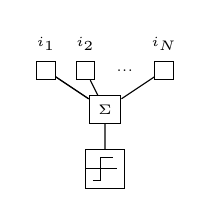
\begin{tikzpicture}[font=\tiny]

	\node (in1) at (-0.75,0) [draw,label=above:{$i_1$}]{};
	\node (in2) at (-0.25,0) [draw,label=above:{$i_2$}]{};
	\node (n) at (0.25,0) []{...};
	\node (inn) at (0.75,0) [draw,label=above:{$i_N$}]{};

	\node (sum) at (0,-0.5) [draw]{$\Sigma$};

	\node (out) at (0,-1.25) [draw,inner sep=7]{};

	\draw (out.west) --  +(0.4,0);
	\draw (out.south west) ++(0.1,0.1) -- ++(0.1,0) -- ++(0,0.3) -- ++(0.15,0);


	\draw (in1) -- (sum) -- (out);
	\draw (in1) -- (sum);
	\draw (in2) -- (sum);
	\draw (inn) -- (sum);
\end{tikzpicture}

\end{tabularx}

Die Feuerschwelle wird benötigt um Beispielsweise boolsche Gatter zu
implementieren, was sonst unmöglich wäre.  Sie kann mit einem Zusätzlichen
Eingang der immer auf 1 gesetzt ist umgesetzt werden.  Das Gewicht dieses
Eingangs entspricht dann der Feuerschwelle.

\subsection{Netze elementarer Perzeptronen}
\begin{figure}[h!]
	\centering
	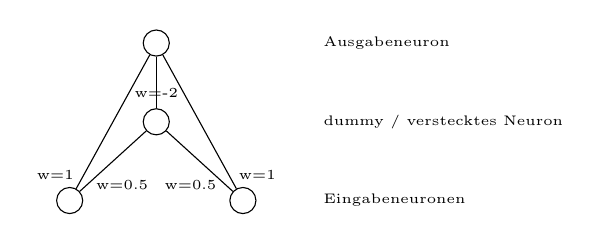
\begin{tikzpicture}[font=\tiny]
	\node (out) at (0,0) [draw,circle]{};
	\node (hidden) at (0,-1) [draw,circle]{};
	\node (in1) at (-1.1,-2) [draw,circle]{};
	\node (in2) at (1.1,-2) [draw,circle]{};

	\draw (out) +(2,0) node[right] {Ausgabeneuron};
	\draw (hidden) +(2,0) node[right] {dummy / verstecktes Neuron};
	\draw (hidden) +(2,-1) node[right] {Eingabeneuronen};

	\draw (in1) -- node[pos=0.1,right]{w=0.5} (hidden);
	\draw (hidden) -- node[pos=0.3]{w=-2} (out);
	\draw (in1) -- node[pos=0.1,left]{w=1}(out);
	\draw (in2) -- node[pos=0.1,left]{w=0.5}(hidden);
	\draw (in2) -- node[pos=0.1,right]{w=1}(out);
\end{tikzpicture}

	\caption{Werbos als Netz von Perzeptronen (XOR-Funktion)}
\end{figure}
\begin{itemize}
	\item Keine versteckte Schicht erlaubt nur linear trennbare Probleme
	\item Eine versteckte Schicht kann zwei konvexe offene oder abgeschlossene Bereiche trennen
	\item Zwei versteckte Schichten können auch nicht-kontinuierliche und nicht zusammenhängende
		Arumentmengen unterteilen. Anzahl und Form hängt von der Anzahl Knoten ab.
\end{itemize}

\subsubsection{Backpropagation}
Fehlerzurückverfolgung bei der Rückwärts durchs Netz Zurückverfolgt wird,
welche Gewichte den grössten Einfluss auf Die Ausgabe haben.
\verweiskurz{2_Gradientenabstieg}

\subsection{Holographisches Perzeptron}
Bei diesen Neuronen bleiben die Phaseninformation im Gegensatz zu den
Perzeptronen erhalten.

\subsection{Kohonennetze}
Kohonennetze sind selbstorganisierend. Sie bestehen aus aneinandergereiten
Neuronen, mit variablen Abstand (Gummiband).

\subsubsection{Beispiel Travelling Salesman}
\begin{itemize}
	\item Neuronen zufällig platzieren
	\item Auswahl zufälliger Stadt
	\item Das am nächsten liegende Neuron nehmen und näher zu dieser Stadt rücken, die anderen Neuronen nachziehen
	\item Wiederholen bis alle Neuronen ihren Platz gefunden haben
\end{itemize}

\subsection{Hopfield}
Das Hopfield-Netz ist geeignet um Muster (Bilder) zu kennen. Dabei wird pro
Pixel ein binäres Neuron verwendet (-1,1).  Dazu erstellt man eine
Korrelationsmatrix, welche alle Muster enthält, es wird nicht gelernt!  Für eine
gute Erkennung sollten die Muster möglichst orthogonal, also linear unabhängig
sein.  Die Berechnung der Korrellationsmatrix funktioniert folgendermassen:

\begin{itemize}
	\item Alle Muster definieren $x_1 = \begin{bmatrix}-1&1&1&1 \end{bmatrix};
			x_2 = \begin{bmatrix}1&1&1&-1\end{bmatrix}$
	\item Energiematrix aus Korrelationsmatrizen erstellen: $M = x_1' x_1 + x_2'
		x_2 =
		\begin{bmatrix}
			 1&-1&-1&-1 \\
			-1& 1& 1& 1 \\
			-1& 1& 1& 1 \\
			-1& 1& 1& 1
		\end{bmatrix} +
		\begin{bmatrix}
			 1& 1& 1&-1\\
			 1& 1& 1&-1\\
			 1& 1& 1&-1\\
			-1&-1&-1& 1
		\end{bmatrix} =
		\begin{bmatrix}
			 2&0&0&-2\\
			 0&2&2& 0\\
			 0&2&2& 0\\
			-2&0&0& 2
		\end{bmatrix}$
	\item Diagonalelemente auf 0 setzen: $M_{i,i} = 0 \rightarrow
		M=\begin{bmatrix}
			 0&0&0&-2\\
			 0&0&2& 0\\
			 0&2&0& 0\\
			-2&0&0& 0
		\end{bmatrix}$
\end{itemize}
\subsubsection{Benötige Anzahl Neuronen}
Pro zu erkennendes Muster ($M$) werden etwa 7 Neuronen ($N$) benötigt.
\begin{itemize}
	\item Bis einige 100 Neuronen: $M_{max} ~ 0.15N$
	\item Für Netze mit sehr grossem N: $M_{max} ~ \frac{0.5N}{log(N)}$
	\item Allgemein gilt $M_{max} < N$
	\item Für $M >= 0.15N$ bilden sich mehr Nebenminimas in denen das Netz
		hängen bleiben kann (Rütteln kann helfen hinauszukommen)
	\item Ab $M > 0.5N$ degenerieren die Energiebarrieren zwischen den Minima,
		wodruch das Netz unbrauchbar wird
\end{itemize}

% vim:tw=80
